\documentclass[10pt,aspectratio=169]{beamer}
\usepackage{graphicx}
\usepackage{booktabs,multirow,tabu}
\usepackage{tikz}
\usepackage{siunitx}
\usepackage[absolute,overlay]{textpos}
\usepackage{adjustbox}
\usepackage{feynmp}
\usepackage{tikz-feynman}
\tikzfeynmanset{compat=1.1.0}

%%%%%%%%%%%%%%%%%%%%%%%%%%%%%%

\usepackage{palatino}             % font
\setbeamercovered{transparent}    % uncover
\usetheme{metropolis}
\usefonttheme{serif}
\hypersetup{
  colorlinks = true,
}
\setbeamertemplate{footline}[frame number]
\setbeamertemplate{navigation symbols}{}
\setbeamerfont{author}{size=\large,series=\bfseries}
\setbeamerfont{date}{size=\normalsize}
\setbeamerfont{institute}{size=\normalsize}
\setbeamerfont{conference}{size=\normalsize,series=\bfseries}
\renewcommand{\instlogoA}{atlas}
\renewcommand{\instlogoB}{sydney}
\graphicspath{{logos/}{figures/}}

%%%%%%%%%%%%%%%%%%%%%%%%%%%%%%

\title{Sydney group update}
\author[]{Sydney group}
\date{\today}
\conference{Australian ATLAS Meeting}

\begin{document}
\begin{frame}\titlepage\end{frame}

%%%%%%%%%%%%%%%%%%%%%%%%%%%%%%%%%%%%%%%%%%%%%%%%%%%%%%%%%%%%%%%

\begin{frame}{Introduction: Four Tops Analysis}
  \begin{figure}
    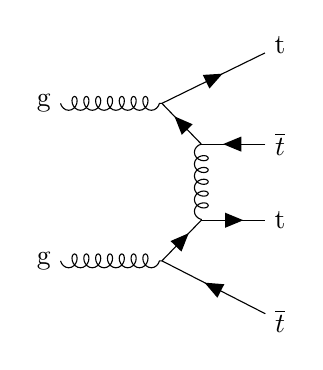
\begin{tikzpicture}
      \begin{feynman}
        % Define the gluons
        \vertex (g1s) {g}; 
        \vertex[right=1.5cm of g1s](g1e);
        
        \vertex[below=2.0cm of g1s](g2s){g};
        \vertex[right=1.5cm of g2s](g2e);

        %Draw all the tops in a line 
        \vertex[right=1.5cm of g1e](tmp); 
        \vertex[above=0.5cm of tmp](t1e) {t}; 
        \vertex[below=0.25cm of tmp](t2e) {\(\overline t\)}; 
        \vertex[below=1.25cm of tmp](t3e) {t}; 
        \vertex[below=2.5cm of tmp](t4e) {\(\overline t\)};
        
        %Draw start of tops 
        \vertex[left=1.0cm of t2e](t2s); 
        \vertex[left=1.0cm of t3e](t3s); 

        \diagram* {
          {[edges=gluon]
            (g1s) -- (g1e), 
            (g2s) -- (g2e), 
            (t2s) -- (t3s),
          }, 
          {[edges=fermion]
            (t2e) -- (t2s) -- (g1e) -- (t1e), 
            (t4e) -- (g2e) -- (t3s) -- (t3e),           
          },
        };
      \end{feynman}
    \end{tikzpicture}
    \bigskip
    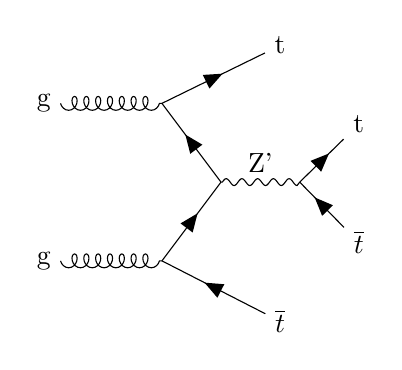
\begin{tikzpicture}
      \begin{feynman}
        % Define the gluons
        \vertex (g1s) {g}; 
        \vertex[right=1.5cm of g1s](g1e);
        
        \vertex[below=2.0cm of g1s](g2s){g};
        \vertex[right=1.5cm of g2s](g2e);

        %Draw all the tops in a line 
        \vertex[right=1.5cm of g1e](tmp); 
        \vertex[above=0.5cm of tmp](t1e) {t}; 
        \vertex[below=2.5cm of tmp](t4e) {\(\overline t\)};         
        
        % Resonance
        \vertex[below=1.0cm of tmp](tmp2); 
        \vertex[left=0.75cm of tmp2](Zs);
        \vertex[right=1.0cm of Zs](Ze); 
        \vertex[right=0.75cm of Ze](tmp3); 

        %Draw start of tops 
        \vertex[above=0.5cm of tmp3](t2e) {t};                   
        \vertex[below=0.5cm of tmp3](t3e) {\(\overline t\)};     

        \diagram* {
          {[edges=gluon]
            (g1s) -- (g1e), 
            (g2s) -- (g2e), 
          }, 
          {[edges=fermion]
            (g1e) -- (t1e), 
            (Zs) -- (g1e), 
            (g2e) -- (Zs),
            (t4e) -- (g2e), 
            (Ze) -- (t2e), 
            (t3e) -- (Ze),
          },
          {[edges=boson]
            (Zs) -- [edge label=Z'](Ze),
          },
        };
      \end{feynman}
    \end{tikzpicture}
    \caption{$t \bar{t} t \bar{t}$ production Feynman diagrams for left) Standard Model right) BSM Top-Philic model}
    \label{fig:Tops}
  \end{figure}
  \begin{itemize}
    \item Within the SM, the 4-top production mode is extremely rare ($\sigma = 12.6^{+5.6}_{-5.2}$fb) and occurs predominantly through gluon fusion.
    \item Some BSM physics models predict a boosting of this cross-section due to modified top quark couplings or the presence of some heavy resonance (Figure \ref{fig:Tops}).  
  \end{itemize}
\end{frame}

\begin{frame}{Introduction: Four Tops Analysis}
  \begin{itemize}
    \item Tops originating from a resonance are expected to be highly boosted and produce fat-jets. 
    \item The analysis group uses these jets in single lepton decay modes to produce reclustered jets (RC-jets). 
    \item The idea is to explore the use of Graph Neural Networks (GNNs) to identify jets originating from resonance tops.
    \item This data science technique has gained a lot of attention recently in HEPP. 
    \item For instance, at Berkeley a group used GNNs to attribute jets to a common parent in the $ttH$ production mode.
  \end{itemize}
\end{frame}

\begin{frame}{What is a Graph Neural Network?}
  \begin{figure}
    \centering 
    \includegraphics[scale=0.25]{Graph}
  \end{figure}

  \begin{itemize}
    \item A Graph Neural Network is a generalized deep learning technique similar to a conventional Neural Network (Deep Layers, Aggregation, Convolution, Pooling etc.)
    \item What makes a GNN unique is that, inherently non-euclidean data can be encoded on graph like data structures where; 
    \begin{itemize}
      \item Nodes - Some object (Particle, Jets) that has attributes ($\eta$, $\phi$, $p_T$, ...)
      \item Edges - Some relation between objects; $\Delta$r, Inv Mass, $\Delta$(*).  
      \item Graph - Some global properties of the graph; Collision Energy, Missing $p_T$, $\phi$...  
    \end{itemize}  
  \end{itemize}

\end{frame}

\begin{frame}{What is a Graph Neural Network?}
  \begin{figure}
    \centering 
    \includegraphics[scale=0.25]{Graph}
  \end{figure}

  An example computation on a graph would follow something like this:
  \begin{itemize}
    \item Edges are updated via a multilayer-perceptron (MLP) ($\phi$) taking as input; current edge state, \textit{sender} and \textit{receiver} node attributes, a global edge value.
    \item 






    \item Nodes connected to other nodes communicate the attribute values to each other through edges 
    \item In a graph all \textit{Sender} nodes send values to a particular \textit{receiving} node.
    \item The node feature value is then updated through some order invariant aggregation function (sum, mean, max).
    \item 


  \end{itemize}










    \item This allows for unordered data to be assigned to nodes arbitrarily, unlike traditional CNN where input order was important. 
    \item More 

  \end{itemize}

\end{frame}






%%%%%%%%%%%%%%%%%%%%%%%%%%%%%%%%%%%%%%%%%%%%%%%%%%%%%%%%%%%%%%%

\end{document}
